\documentclass[a4paper,12pt]{article}
\usepackage[utf8]{inputenc}
\usepackage{graphicx}
\usepackage[english]{babel}
\usepackage{geometry}
\usepackage{setspace}
\usepackage{minted}
\usepackage{booktabs}
\usepackage{amsmath}
\usepackage[table]{xcolor}
\usepackage{array}
\usepackage{hyperref}

\geometry{margin=1in}
\onehalfspacing

\begin{document}

\begin{titlepage}
    \begin{center}
        % Logos
        \vspace*{-1cm}
        \makebox[\textwidth]{%
            
\includegraphics[width=3cm]{images/logo_purple.png}\hfill
            
\includegraphics[width=3cm]{images/logo_blue.png}
        }
        \vspace{2cm}
        
        % Title
        {\Large \textbf{Boolean Model of ERBB-Driven G1/S Transition}} \\[1cm] 
        
        % Subtitle
        \textit{Module: Modélisation et simulation S8} \\[1.5cm]
        
        % Add more vertical space to center the image better
        \vspace{2cm}
        
        % Add the diagram here
        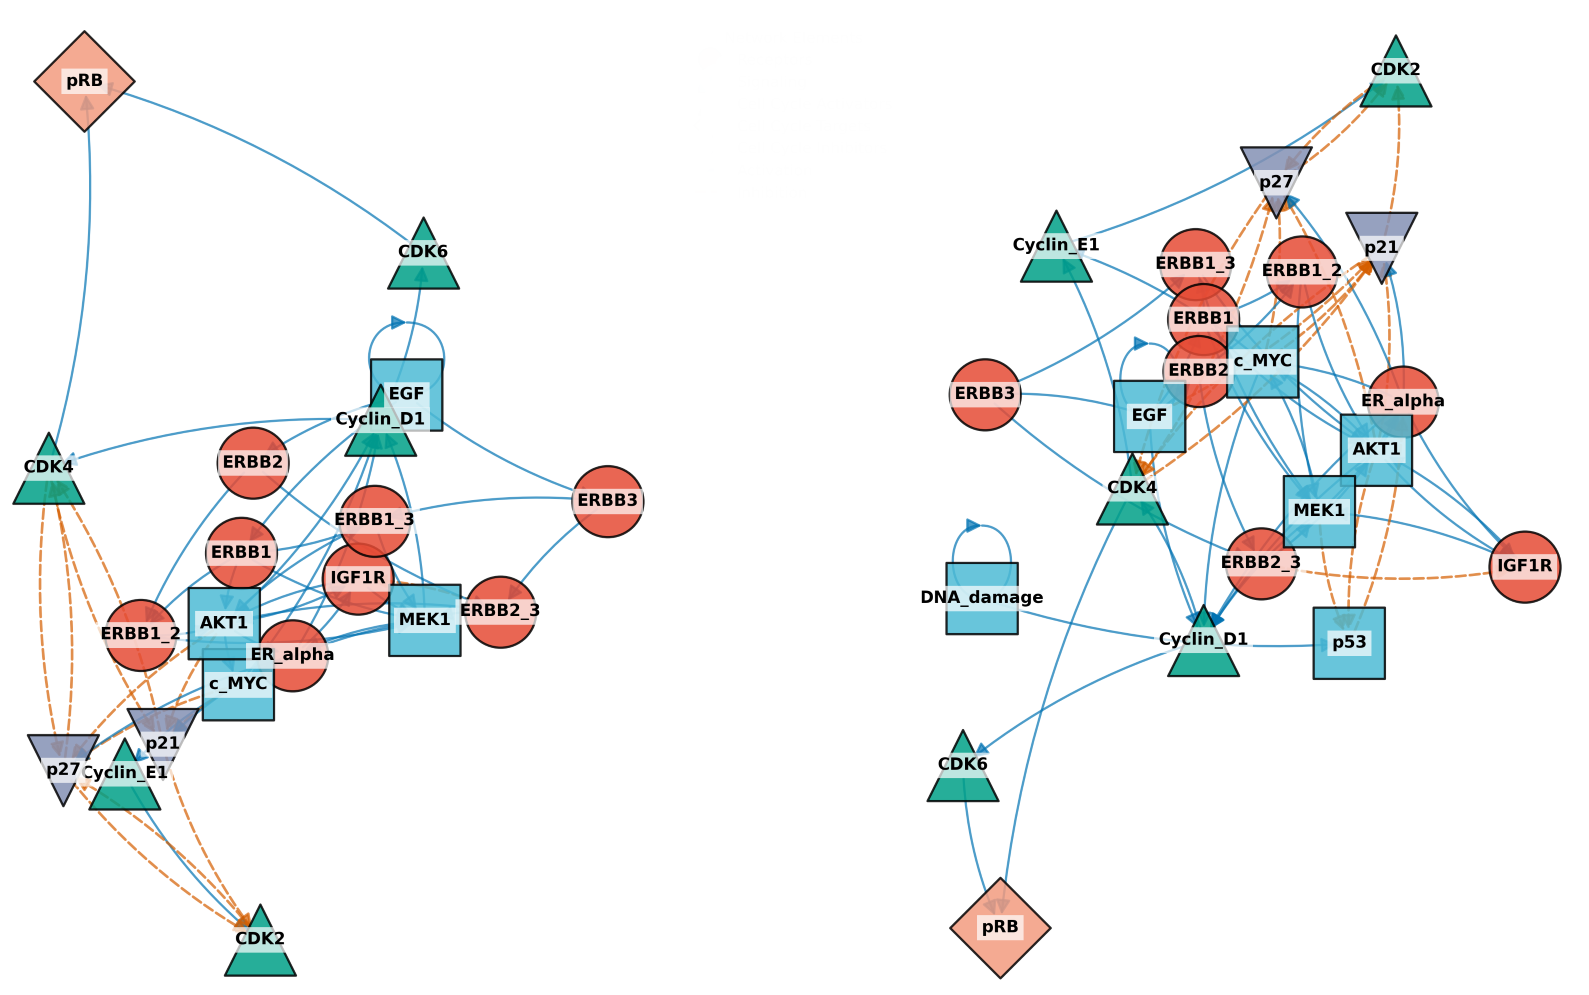
\includegraphics[width=0.8\textwidth]{images/front_page_diagram.png} \\[1.5cm]
        
        \vfill % still push authors to bottom but leave less space

        \textbf{Authors} \\[0.5cm]
        \textsc{Raul DURAN DE ALBA, Denys BURYI}

    \end{center}
\end{titlepage}

\newpage

\section{Introduction}
The ErbB (HER) signaling pathway is a critical regulator of cell proliferation and survival, with particular relevance in breast cancer. Overexpression of transmembrane tyrosine kinase (ERBB2) specifically is connected with adverse prognosis, and so it is targeted by monoclonal antibody trastuzumab in addition to the primary therapy. Unfortunately some cancer cells develop the \textit{de novo} resistance to this antibody. In the publication by Sahin et al. (2009), the authors presented a Boolean network approach to model ErbB dynamics and experimental testing of the resulting network in order to try to find alternative therapeutic targets for such \textit{de novo} trastuzumab resistant cancer cells.

Our project builds on that work by first reproducing the original Boolean network framework to confirm the published results regarding stable states and attractors. We then extend that analysis using new computational


\section{Original paper}

The authors began with the selection of a specific cell line exhibiting both high ERBB2 expression and resistance to trastuzumab treatment—essential characteristics for identifying alternative therapeutic targets for treatment-resistant cells. Initially focusing on the G1/S cell-cycle checkpoint, the researchers established phosphorylation of pRB as their primary readout, which serves as a marker for transition into S-phase. Through validation with Western blot and Reverse Phase Protein Arrays (RPPA), they confirmed that pRB phosphorylation reliably reflected G1/S progression in the HCC1954 cell line.

Based on literature review, the research team constructed an initial Boolean network comprising 18 proteins, including ERBB1/2/3, AKT1, MEK1, c-MYC, ER-$\alpha$, various Cyclins, and CDKs. This network encoded regulatory logic through Boolean rules and was implemented in GINsim modeling software. To predict potential inhibitors of G1/S progression, the team performed \textit{in silico} knockdowns of network proteins, followed by experimental validation through \textit{in vitro} siRNA knockdowns in the HCC1954 cell line, targeting both individual proteins and combinations (e.g., EGFR + ERBB2).

Subsequent comparative analysis revealed discrepancies between the real cell responses and Boolean model predictions regarding which knockdowns induced significant decreases in pRB phosphorylation. This led to refinement of the network rules, particularly making CycD1 activation requirements more stringent. Following these adjustments, the revised model's predictions largely aligned with experimental results, though inconsistencies remained regarding CycE1.

To address remaining discrepancies and investigate cell line-specific regulatory mechanisms, the researchers employed reverse phase protein arrays to quantify activation and expression levels of network components following both individual and combinatorial protein knockdowns. This comprehensive approach confirmed many literature-documented interactions while also identifying novel cell line-specific relationships. Interestingly, the Boolean network correctly predicted most interactions, despite occasional discrepancies in edge directions—a common challenge when inferring regulatory relationships from biological literature. This methodology demonstrated the feasibility of reverse-engineering protein-level Boolean networks, though some discrepancies remained unresolved despite this sophisticated approach.

\subsection{Reproducing the original results}

Similar to the authors, initially we implemented a Boolean model of the ERBB receptor signaling network with rules based on known pathway interactions from literature. Key growth factor receptors (EGFR/ERBB1, ERBB2/HER2, ERBB3, IGF1R) form the input layer, activating downstream PI3K--AKT and RAS--MEK--ERK pathways. These cascades converge on cell-cycle regulators such as the proto-oncogene c-MYC and cyclin D1, ultimately controlling phosphorylation of the retinoblastoma protein pRB -- the Boolean proxy for G1/S transition (pRB phosphorylated = cell-cycle entry). The initial Boolean rules were derived from experimental evidence and assumed some redundancy in mitogenic signaling. For example, Cyclin D1 was assumed ON if any major upstream signal was present: AKT1 or MEK1 activity, estrogen receptor-$\alpha$ (ER-$\alpha$) signaling, or c-MYC could each independently induce cyclin D1 (logical OR). This captured the idea that multiple pathways can upregulate cyclin D1 expression. Other rules included CDK4 activation requiring cyclin D1 and absence of CDK inhibitors p21/p27, CDK6 requiring cyclin D1, and so on. Table \ref{tab:boolean_rules} highlights the original versus refined logic for all nodes in the network.

\begin{table}[ht!]
    \centering
    \begin{tabular}{lp{0.65\textwidth}}
        \toprule
        \textbf{Target} & \textbf{Logical rules for the activation of target} \\ 
        \midrule
        ERBB1 & EGF \\ 
        ERBB2 & EGF \\ 
        ERBB3 & EGF \\ 
        ERBB1\_2 & ERBB1 $\wedge$ ERBB2 \\ 
        ERBB1\_3 & ERBB1 $\wedge$ ERBB3 \\ 
        ERBB2\_3 & ERBB2 $\wedge$ ERBB3 \\ 
        IGF1R & (ER-$\alpha$ $\vee$ AKT1) $\wedge$ $\neg$ERBB2\_3 \\ 
        ER-$\alpha$ & AKT1 $\vee$ MEK1 \\ 
        c-MYC & AKT1 $\vee$ MEK1 $\vee$ ER-$\alpha$ \\ 
        AKT1 & ERBB1 $\vee$ ERBB1\_2 $\vee$ ERBB1\_3 $\vee$ ERBB2\_3 $\vee$ IGF1R \\ 
        MEK1 & ERBB1 $\vee$ ERBB1\_2 $\vee$ ERBB1\_3 $\vee$ ERBB2\_3 $\vee$ IGF1R \\ 
        CDK2 & Cyclin E1 $\wedge$ $\neg$p21 $\wedge$ $\neg$p27 \\ 
        CDK4 & Cyclin D1 $\wedge$ $\neg$p21 $\wedge$ $\neg$p27 \\ 
        CDK6 & Cyclin D1 \\ 
        Cyclin D1 & AKT1 $\vee$ MEK1 $\vee$ ER-$\alpha$ $\vee$ c-MYC \\ 
        Cyclin D1* & ER-$\alpha$ $\wedge$ c-MYC $\wedge$ (AKT1 $\vee$ MEK1) \\ 
        Cyclin E1 & c-MYC \\ 
        p21 & ER-$\alpha$ $\wedge$ $\neg$AKT1 $\wedge$ $\neg$c-MYC $\wedge$ $\neg$CDK4 \\ 
        p27 & ER-$\alpha$ $\wedge$ $\neg$CDK4 $\wedge$ $\neg$CDK2 $\wedge$ $\neg$AKT1 $\wedge$ $\neg$c-MYC \\
        pRB & (CDK4 $\wedge$ CDK6) $\vee$ (CDK4 $\wedge$ CDK6 $\wedge$ CDK2) \\
        \bottomrule
    \end{tabular}
    \caption{Boolean rules for the activation of each component of the network. The refined rules for Cyclin D1 are shown with "*". Symbols "$\wedge$": AND, "$\vee$": OR and "$\neg$": NOT.}
    \label{tab:boolean_rules}
\end{table}

Then we analyzed the network dynamics by:
\begin{itemize}
    \item Identifying stable states using \texttt{analyze\_stable\_states(model)}
    \item Trying to calculate all attractors (including cycles) using \texttt{analyze\_attractors(model)}
\end{itemize}
We found 3 stable states for the original network and identified preliminary therapeutic targets based on the code in \texttt{src.analysis.drug\_targets.py}. This mirrors the study's analysis of network states that lead to G1/S transition.

To validate the model, we simulated the effect of various gene knockouts and compared the outcomes to experimental data from Sahin et al. (2009) . The focus was on key regulators of G1/S: cyclin D1, c-MYC, ER-$alpha$, CDK4/6, cyclin E1, and major upstream signals. In the laboratory, silencing any of Cyclin D1, c-MYC, CDK4/6, Cyclin E1, or ER-$alpha$ is known to strongly reduce pRB phosphorylation and prevent G1/S transition . In contrast, knocking out individual upstream receptors (EGFR, HER2) or single pathway components (AKT1, MEK1) does not fully block G1/S due to pathway redundancy . Table 2 shows the most important comparisons:

\begin{table}[hb!]
    \centering
    \begin{tabular}{lp{0.2\textwidth}p{0.2\textwidth}p{0.2\textwidth}}
        \toprule
        \textbf{Gene Knockout} & \textbf{Experimental Outcome} & \textbf{Original Model Prediction} & \textbf{Refined Model Prediction} \\ 
        \midrule
        ER-$\alpha$ & G1/S blocked & G1/S proceeds & G1/S blocked \\ 
        c-MYC & G1/S blocked & G1/S partially proceeds & G1/S blocked \\
        \bottomrule
    \end{tabular}
    \caption{Knockout Effects on G1/S Transition: Experiment vs Model (pRB phosphorylation as G1/S readout)}
    \label{tab:knockout_effects}
\end{table}

Simulations of the original model revealed clear discrepancies: the model incorrectly predicted that knocking out ER-$\alpha$ would have no effect on pRB ($\sim$67\% of cell-cycle activity remained, identical to wild-type), and that c-MYC knockdown would only partially reduce pRB phosphorylation (some stable states still had pRB=1) -- in stark contrast to experiments where both knockdowns abolish pRB phosphorylation~\cite{Sahin2009}. In our simulations, the original model yielded 3 stable states even for the ER-$\alpha$ or c-MYC knockout, with one or more states still showing active cyclin E/CDK2 and phosphorylated pRB (indicating cell-cycle entry). The root cause was evident: cyclin D1 could still be activated via redundant inputs (AKT or MEK) in the absence of ER-$\alpha$ or c-MYC, allowing pRB to be phosphorylated via CDK4/6. This is a model failure, since biologically ER-$\alpha$ and c-MYC are each required for sufficient cyclin D1 expression in the cellular context.

Other knockout simulations of the original network were more consistent with data. For example, knocking out Cyclin D1 itself or CDK4 correctly resulted in pRB remaining unphosphorylated (G1 arrest) in silico, matching experiments . Likewise, the model correctly showed that no single EGFR/ERBB family receptor knockout could completely stop G1/S (since parallel receptors compensate) . An interesting case was IGF1R knockout: experimentally this also causes G1/S block in the studied cells , but the original model produced two possible stable states -– one with pRB off (arrest) and one with pRB on -– an ambivalent prediction reflecting uncertainty in how IGF1R crosstalk was represented. This indicated room for improvement in that part of the network as well. Overall, however, the most glaring inconsistencies centered on cyclin D1 regulation via ER-$alpha$ and c-MYC.

\subsubsection{Logic refinement}

To resolve the inconsistencies, we followed the approach of the authors and refined the Boolean logic of the network. The key change was that cyclin D1 expression requires combined inputs from estrogen/ER-$alpha$ signaling and c-MYC, in addition to mitogenic pathway activation. Biologically, this makes sense: estrogen-responsive cells need both hormone signaling (ER-$alpha$ → cyclin D1 transcription) and growth factor-induced transcriptional programs (via c-MYC and MAPK/AKT) to accumulate enough cyclin D1 for pRB phosphorylation~\cite{Louie2017}. We therefore replaced the cyclin D1 rule with a more stringent one (Table 1 above): cyclin D1 is ON if and only if ER-$alpha$ and c-MYC are both active, and at least one of AKT1 or MEK1 is active . In logical terms, the new rule is:

\begin{equation}
\text{Cyclin D1} = \text{ER-$\alpha$} \wedge \text{c-MYC} \wedge (\text{AKT1} \vee \text{MEK1})
\end{equation}

This refinement eliminated the redundant “either-or” inputs from the original rule , making cyclin D1 induction contingent on cooperative signaling. It reflects the experimental observation that ER-$alpha$ or c-MYC knockdown alone should be sufficient to prevent cyclin D1 upregulation and cell-cycle entry. 
We tested several alternative logic combinations for cyclin D1 and its regulators (varying the requirements on ER-$alpha$ and c-MYC) and found that the chosen rule best reproduced the experimental phenotypes. Importantly, this change did not contradict any prior assumptions for cases the original model already got right –- it was a conservative refinement that only changed one rule that was too loose. No other node rules required adjustment in this round of refinement, since the mismatch with data was specific to cyclin D1 regulation.

\subsubsection{Validation of the refined model}
The refined model was subjected to the same analyses as the original to ensure that the discrepancies were resolved and that no new ones were introduced. Crucially, the refined Cyclin D1 rule corrected the predictions for ER-$\alpha$ and c-MYC perturbations. In silico knockdown of ER-$\alpha$ now resulted in cyclin D1 staying OFF (since the AND condition with c-MYC fails), leading to loss of CDK4/6 activity and pRB remaining unphosphorylated -- accurately predicting G1 arrest as observed experimentally~\cite{Sahin2009}. Similarly, c-MYC knockdown now leaves cyclin D1 OFF and the model shows complete G1/S blockage, matching the empirical outcome~\cite{Sahin2009}. 

Quantitatively, the ``cell-cycle activity'' metric for these knockouts dropped to 0\% (for c-MYC) or a very low value ($\sim$22\% for ER-$\alpha$, reflecting a minor residual in one attractor) in the refined model, whereas these were $\sim$67\% in the original model (essentially wild-type levels) as shown in Table~\ref{tab:knockout_effects}. In effect, the refined network now encodes that both ER-$\alpha$ and c-MYC are indispensable -- knocking out either is as effective as knocking out cyclin D1 itself at preventing G1/S. This is in perfect concordance with the experimental data.
The ambiguous case of IGF1R knockout remained: the refined model, like the original, produces two stable states for IGF1R loss (one with pRB phosphorylated, one unphosphorylated), indicating a still unresolved model ambiguity in that branch. This suggests that additional refinement or data (e.g. considering cross-talk between IGF1R and ERBB signaling) may be needed to fully capture the role of IGF signaling in this context.

In summary no new inconsistencies were introduced by the cyclin D1 rule change -– all other network behaviors and stable states remained biologically reasonable. The number of stable states in the refined model remained three, as in the original, indicating that the overall dynamical repertoire of the network was preserved. However, the composition of those states shifted to reflect the fact that the cell needs both ER-$\alpha$ and c-MYC to activate cyclin D1 and enter S-phase. 

\subsubsection{Phenotype control via permanent perturbations}

Following the approach described by Benes et al.~\cite{Benes2023}, we investigated how permanent perturbations could control network phenotypes, specifically focusing on inducing cell cycle arrest. Unlike transient knockdowns, permanent perturbations fix the value of specific nodes to either ON or OFF, mimicking sustained therapeutic interventions such as targeted inhibitors or gene expression modulators. In our analysis, cell cycle arrest was defined as the absence of pRB phosphorylation and inactivation of CDK2, CDK4, and CDK6.

We systematically evaluated single-node perturbations by fixing each component to either ON or OFF, then analyzing the resulting stable states. In the original model, few single perturbations induced complete cell cycle arrest, consistent with the redundancy in mitogenic signaling pathways. The refined model showed increased sensitivity to perturbations targeting core regulators of Cyclin D1, with knockouts of ER-$\alpha$ and c-MYC reliably causing arrest as observed experimentally. This confirms that the refined rules better represent the biological dependencies required for G1/S transition.

Extending our analysis to combination perturbations, we tested therapeutically relevant combinations including dual EGFR/HER2 inhibition, combined PI3K/MAPK pathway blockade, and triple combinations targeting receptors and downstream effectors. Several combinations were particularly effective at inducing arrest across all model variants:

\begin{itemize}
    \item Combined AKT1 and MEK1 inhibition, blocking both major mitogenic signaling branches
    \item ERBB2 inhibition combined with MEK1 blockade, mimicking a clinically relevant drug combination
    \item Triple combinations targeting ERBB2, AKT1, and MEK1 simultaneously
\end{itemize}

\begin{figure}[!htb]
    \centering
    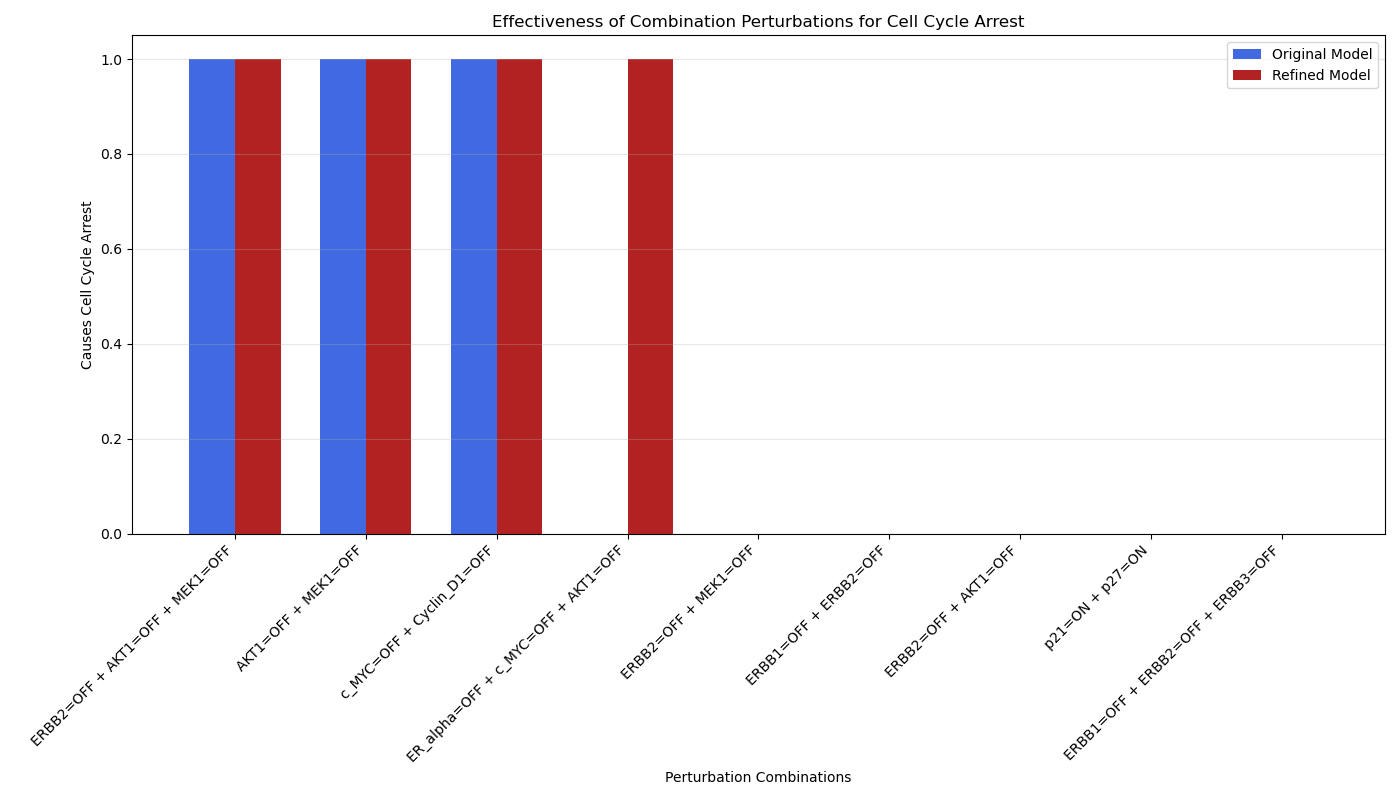
\includegraphics[width=\textwidth]{images/combination_perturbations.png}
    \caption{Effectiveness of combination perturbations for inducing cell cycle arrest across original and refined model variants. Red bars represent combinations that cause arrest in the refined model, blue bars in the original model. Most effective combinations include dual pathway inhibition (AKT1+MEK1) and receptor plus pathway targeting (ERBB2+MEK1).}
    \label{fig:combination_perturbations}
\end{figure}

Interestingly, some combinations effective in the refined model were ineffective in the original model, highlighting how improved network logic reveals intervention targets that would otherwise be missed. For example, the combined targeting of ER-$\alpha$ and c-MYC showed divergent effects between models, with only the refined model correctly predicting cell cycle arrest. Our combinatorial perturbation analysis also identified potentially synergistic targets that could overcome pathway redundancy and resistance mechanisms in ERBB2-overexpressing cells, as shown in Figure~\ref{fig:combination_perturbations}.

The most effective combination perturbations (consistently causing arrest in both models) were:
\begin{itemize}
    \item ERBB2 = OFF + AKT1 = OFF + MEK1 = OFF (triple inhibition)
    \item AKT1 = OFF + MEK1 = OFF (dual pathway inhibition)
    \item c-MYC = OFF + Cyclin D1 = OFF (transcription factor and effector inhibition)
\end{itemize}

This computational analysis of permanent perturbations provides a rational basis for designing combination therapies in trastuzumab-resistant breast cancer, suggesting specific molecular targets that could be inhibited to enforce cell cycle arrest even when single-target approaches fail.

\subsection{LogicGep}

Initially we intended to apply the LogicGep method (\cite{Zhang2024}) to our Boolean model, but because it requires time-series data for training, we could not proceed with this approach. The original paper by Sahin et al. (2009) did not provide time-series data for the model components, and we were unable to find suitable datasets in the literature.  
So instead we used the principles of the approach and additional, newer literature on the subject to extend the refined model (Tean et al.\cite{Tian2009}, Das et al. \cite{Das2025}, Vivekanandhan et al. \cite{Vivekanandhan2022}). The further refined logic rules can be found in the Table below:

\begin{table}[htbp!]
    \centering
    \begin{tabular}{lp{0.65\textwidth}}
        \toprule
        \textbf{Target} & \textbf{LogicGep-Refined Logical Rules} \\ 
        \midrule
        AKT1 & ERBB1 $\vee$ ERBB1\_2 $\vee$ ERBB1\_3 $\vee$ ERBB2\_3 $\vee$ IGF1R \\ 
        CDK2 & Cyclin\_E1 $\wedge$ $\neg$p21 $\wedge$ $\neg$p27 \\ 
        CDK4 & Cyclin\_D1 $\wedge$ $\neg$p21 $\wedge$ $\neg$p27 \\ 
        CDK6 & Cyclin\_D1 \\ 
        Cyclin\_D1 & EGF $\wedge$ ER\_alpha $\wedge$ c\_MYC $\wedge$ (AKT1 $\vee$ MEK1) \\ 
        Cyclin\_E1 & CDK4 $\wedge$ c\_MYC \\ 
        DNA\_damage & DNA\_damage \\ 
        EGF & EGF \\ 
        ERBB1 & EGF \\ 
        ERBB1\_2 & ERBB1 $\wedge$ ERBB2 \\ 
        ERBB1\_3 & ERBB1 $\wedge$ ERBB3 \\ 
        ERBB2 & EGF \\ 
        ERBB2\_3 & ERBB2 $\wedge$ ERBB3 \\ 
        ERBB3 & EGF \\ 
        ER\_alpha & $\neg$p53 $\wedge$ (AKT1 $\vee$ MEK1) \\ 
        IGF1R & $\neg$ERBB2\_3 $\wedge$ (AKT1 $\vee$ ER\_alpha) \\ 
        MEK1 & ERBB1 $\vee$ ERBB1\_2 $\vee$ ERBB1\_3 $\vee$ ERBB2\_3 $\vee$ IGF1R \\ 
        c\_MYC & ER\_alpha $\wedge$ (AKT1 $\vee$ MEK1) \\ 
        p21 & ER\_alpha $\wedge$ $\neg$AKT1 $\wedge$ $\neg$CDK4 $\wedge$ $\neg$EGF $\wedge$ $\neg$c\_MYC \\ 
        p27 & ER\_alpha $\wedge$ $\neg$AKT1 $\wedge$ $\neg$CDK2 $\wedge$ $\neg$CDK4 $\wedge$ $\neg$c\_MYC \\ 
        p53 & DNA\_damage $\vee$ $\neg$(AKT1 $\wedge$ MEK1) \\ 
        pRB & (CDK4 $\wedge$ CDK6) $\vee$ (CDK2 $\wedge$ CDK4 $\wedge$ CDK6) \\
        \bottomrule
    \end{tabular}
    \caption{LogicGep-refined Boolean rules for the ERBB signaling network. Key refinements include: direct EGF dependence for Cyclin D1, CDK4 requirement for Cyclin E1, dependency of c-MYC on ER-$\alpha$, and introduction of p53-mediated stress response. Symbols "$\wedge$": AND, "$\vee$": OR and "$\neg$": NOT.}
    \label{tab:logicgep_rules}
\end{table}

We then performed the \textit{in silico} knockout analysis on the all three models (\ref{fig:logicgep_model_comparison}) and compared the results. The results of the analysis are shown in Table \ref{tab:knockout_effects}. The LogicGep-refined model shows more conditions when cell cycle arrest is achieved. It is possible that this model has found some novel therapeutic targets, but without the ability to experimentally validate the rules we used, it's hard to gage the veracity of the model. Lastly, we have vizualized the refined model in the figure \ref{fig:logicgep_model_vizualization}. 
\begin{figure}[!htbp]
    \centering
    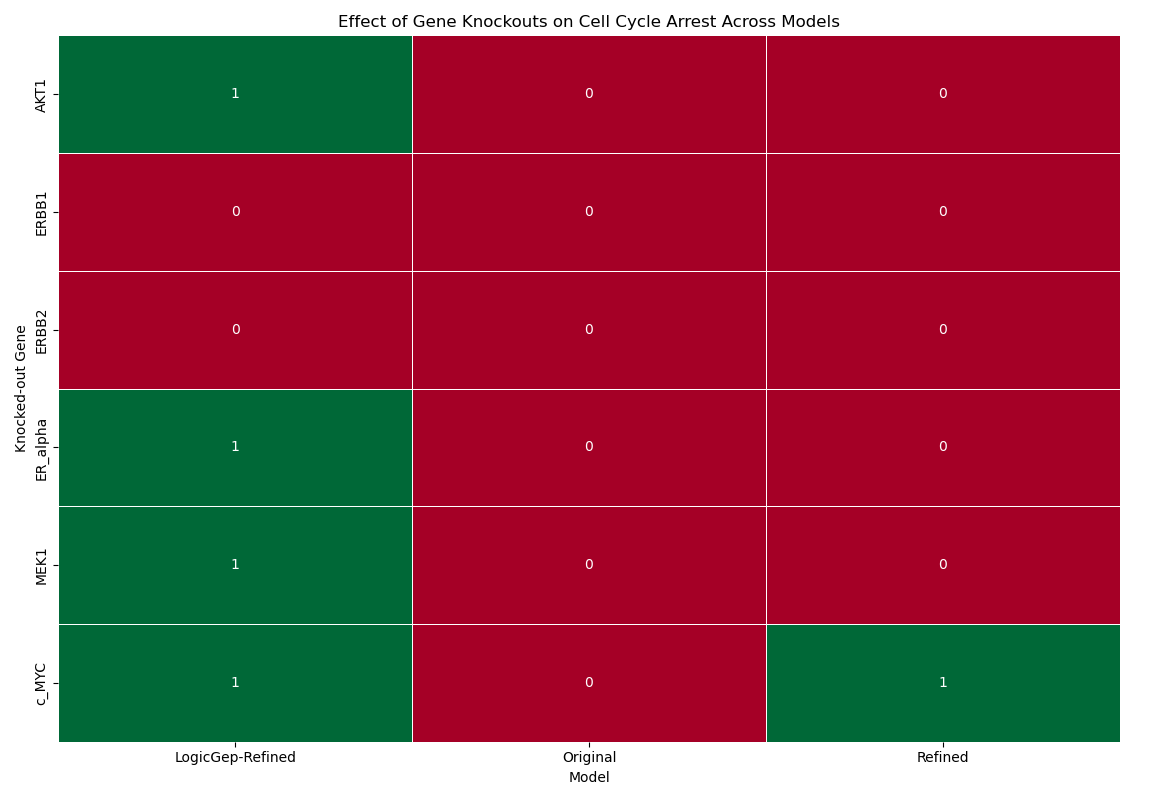
\includegraphics[width=\textwidth]{images/logicgep_model_comparison.png}
    \caption{Effect of on cell cycle arrest across the original, refined, and LogicGep-refined models. Green represents cell cycle arrest. The LogicGep-refined model shows more conditions when cell cycle arrest is achieved.}
    \label{fig:logicgep_model_comparison}
\end{figure}

\begin{figure}[!htbp]
    \centering
    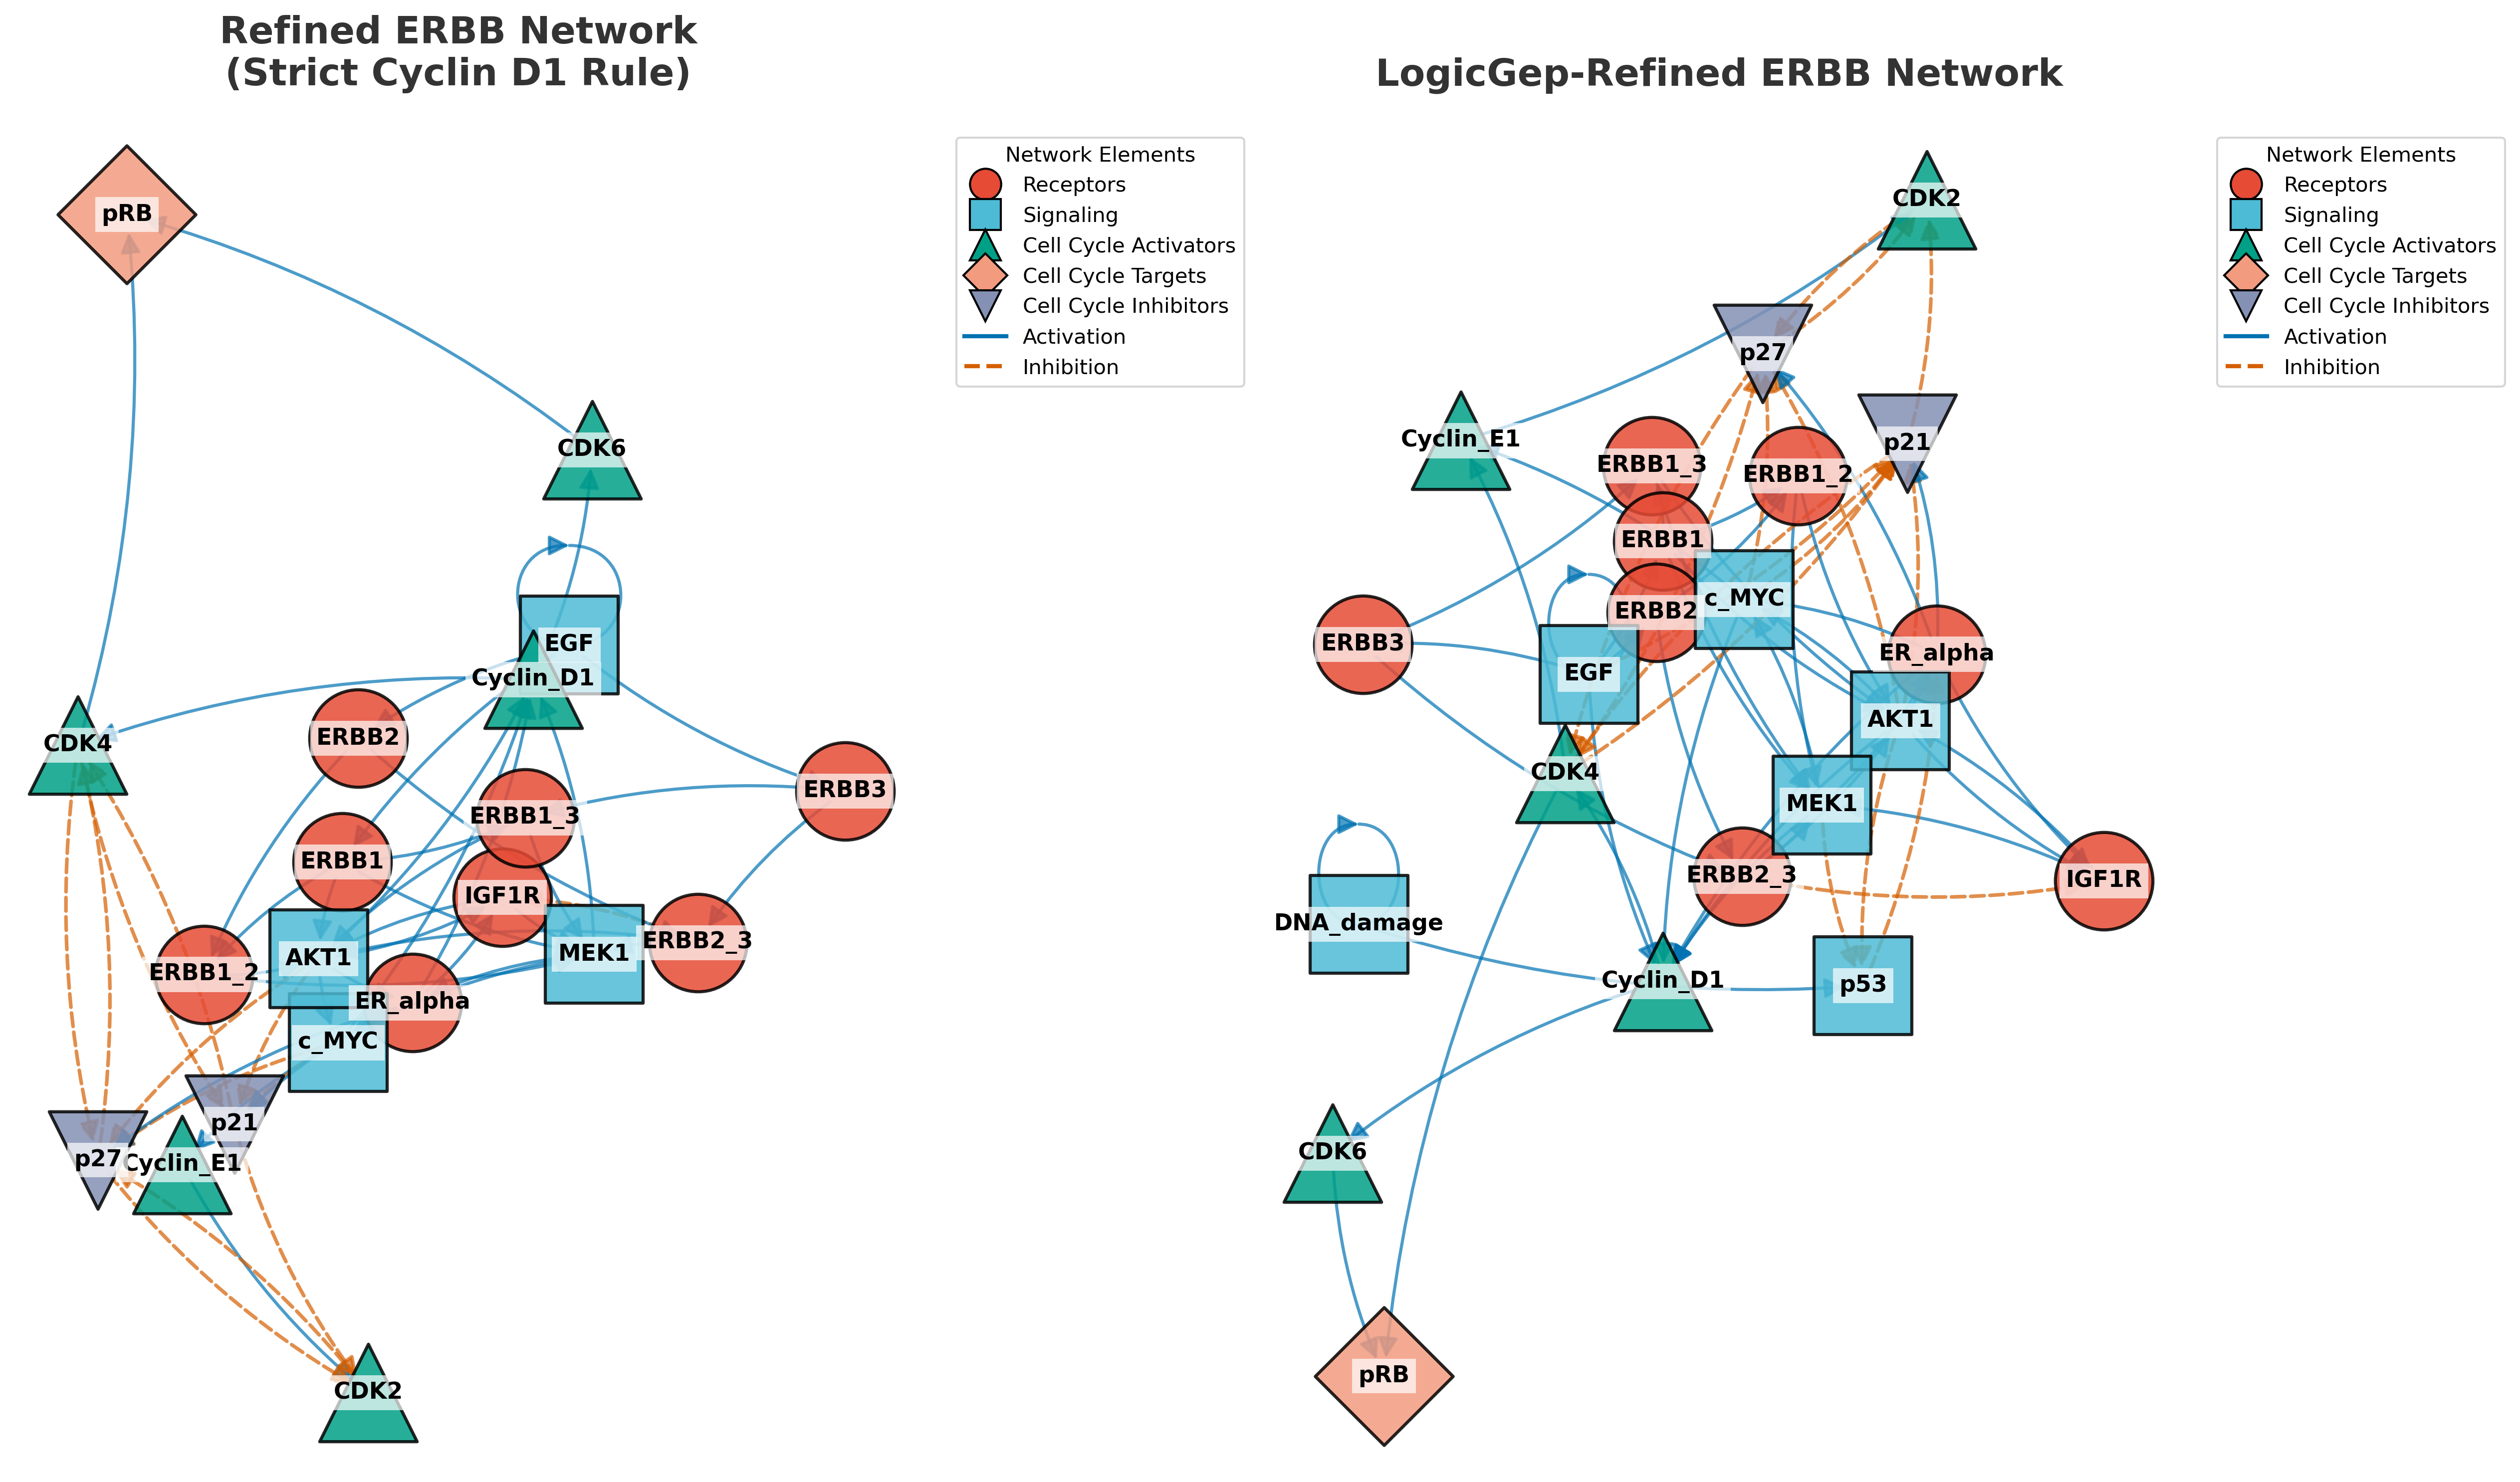
\includegraphics[width=\textwidth]{images/ERBB_logicgep_network.png}
    \caption{Vizualization of the strict CycD1 rule (left) and the LogicGep-refined model (right).}
    \label{fig:logicgep_model_vizualization}
\end{figure}


\clearpage


\begin{thebibliography}{99} 
\bibitem{Sahin2009} Sahin, Ö., Fröhlich, H., et al. (2009). Modeling ERBB receptor-regulated G1/S transition to find novel targets for de novo trastuzumab resistance. BMC Systems Biology, 3(1), 1-20.
\bibitem{Louie2017} Louie, M. C., \& Sevigny, M. B. (2017). Steroid hormone receptors as prognostic markers in breast cancer. American Journal of Cancer Research, 7(8), 1617-1636.
\bibitem{Benes2023} Benes, P., Fauré, A., de Jong, H., Paulevé, L., \& Šafránek, D. (2023). Phenotype control using permanent perturbations computed via reachability analysis. In Computational Methods in Systems Biology (pp. 23-40). Springer, Cham. https://doi.org/10.1007/978-3-031-42697-1\_2
\bibitem{Zhang2024} Zhang, H., Wu, X., Huang, T., Pandey, J., Li, S., \& Rajapakse, J. C. (2024). LogicGep: Logic network optimization through genetic evolution of policy. Briefings in Bioinformatics, 25(4), bbae286. https://doi.org/10.1093/bib/bbae286
\bibitem{Tian2009} Tian, T., Olson, S., Whitacre, J. M., \& Harding, A. (2009). The origin of cancer associated errors in gene expression logic. Cell, 137(2), 225-234. https://doi.org/10.1016/j.cell.2009.05.002
\bibitem{Das2025} Das, G. M., Oturkar, C. C., \& Menon, V. (2025). Interaction between Estrogen Receptors and p53: A Broader Role for Tamoxifen? Endocrinology, 166(3), bqaf020. https://doi.org/10.1210/endocr/bqaf020
\bibitem{Vivekanandhan2022} Vivekanandhan, S., \& Knutson, K. L. (2022). Resistance to Trastuzumab. Cancers, 14(20), 5115. https://doi.org/10.3390/cancers14205115
% Add more \bibitem entries as needed
\end{thebibliography}

\end{document}  % Fixed: added curly braces